\section{WSNet}

TODO: write introduction
wanted to check results, first implement them, check for deviations, make experiments, look at explainability (maybe)

\subsection{Code availability and reproduction of the results}

Although the code for WSNet \cite{Oota_2023_WACV} is stated to be publicly available, a closer inspection of the linked GitHub repository shows that this is only partially the case. A lack of documentation makes using the code hard, especially since it seems to contain multiple errors, making it only suitable as a base for new code.

In this project's scope, the code was used to create runnable models again. Unfortunately, the classes of the wounds are not available, making it impossible to perform pre-training as described in the original paper \cite{Oota_2023_WACV}. In total, there are eight models available: A local model and a combined global-local model for each of the segmentation models: Unet, PSPNet, FPN, and LinkNet. The Python library used for the segmentation models is \texttt{segmentation\_models} \cite{SegmentationModels}. The implementation process showed some differences from the described model architecture. In particular, it was claimed that the wound images were split up in parts of 48\,px times 48\,px. However, three of the four models, all besides PSPNet, only allow input sizes divisible by 32, and the code in GitHub showed a size of 64\,px was used. Another difference between the available code and the paper is that it is claimed that augmentation is not performed on the test images, which is not the case.

Information about the training, validation and test set size is not given in the paper or code. However, the code reveals that the train and validation sets were just the first x\,\% of the dataset, and no randomisation was used to separate the test set as it is usually done. In this project's scope, a split of 70\,\% training, 15\,\% validation and 15\,\% test data is used.

Because the data training for the wound-specific pre-training is not available, the results can only be compared for imagenet pre-training.


\begin{itemize}
	\item problem with imagenet pre-training with mobilenet: input size for patches is not available, instead the default size of 224 is used, which might impact results negatively
\end{itemize}


\subsection{Comparison of the achieved performance}

\begin{table}[htb!]
	\centering
	\begin{tabular}{l||c | c | c | c | c | c | c | c|}
	& \multicolumn{2}{|c|}{Unet} & \multicolumn{2}{|c|}{LinkNet} & \multicolumn{2}{|c|}{PSPNet} & \multicolumn{2}{|c|}{FPN} \\
	\hline
	& IoU & Dice & IoU & Dice & IoU & Dice & IoU & Dice \\
	\hline\hline
	\textbf{Local model} & 0.359 & 0.523 & 0.398 & 0.564 & 0.373 & 0.538 & 0.408 & 0.574 \\	
	\textbf{Global model} & 0.504 & 0.668 & 0.631 & 0.772 & 0.458 & 0.627 & 0.632 & 0.772 \\
	\textbf{Global-Local model} & 0.495 & 0.658 & 0.618 & 0.763 & 0.476 & 0.642 & 0.612 & 0.758\\
	\end{tabular}
	\caption{IoU-Scores and Dice Coefficients for the four different models with each Global-Local, Global and Local architecture. The backbone used is mobilenet.}
\end{table}

\begin{table}[htb!]
	\centering
	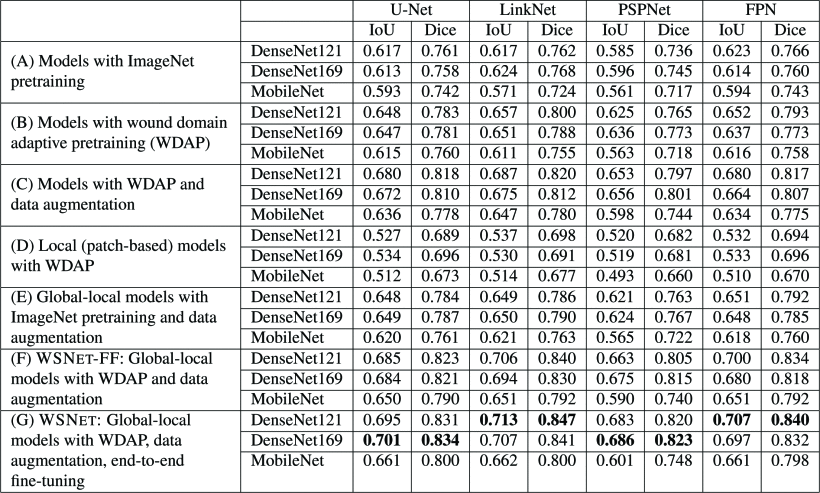
\includegraphics[width=\textwidth]{fig/wsnet-results.png}
	\caption{Results reported by \citeauthor{Oota_2023_WACV} \cite{Oota_2023_WACV}.}
\end{table}

\begin{itemize}
	\item results are comparable with results reported in paper, slightly lower scores
	\item e.g. Unet IoU score 0.495 with my code, 0.620 in paper (dice score 0.761 vs 0.658)
	\item others are closer (LinkNet 0.618 from me vs 0.621 in paper, dice 0.763 in paper and for me)
	\item maybe differences in training size
	\item most important thing: the global-local model does not improve about global model (or at least less than reported in paper)
	\item but they are still way more computationally expensive because you need to train two models instead of one
	\item as discussed before, an improvement indicates that something is going on with 48\,px context size
	\item the results reported by \citeauthor{Oota_2023_WACV} are shown in figure
\end{itemize}

\subsection{Experiments with the activation function}

\begin{itemize}
	\item code shows use of sigmoid as activation function
	\item literature of the model reports ReLU more frequently, thus it was tested as alternative to sigmoid
	\item no clear trend of one being clearly better for all models and architectures
\end{itemize}

\subsection{Combination of different architectures}

\begin{itemize}
	\item used model architectures localize signals differently by design
	\item if the patch size really does play a significant role, maybe it makes sense to combine different architecture sizes?
\end{itemize}
